\begin{figure}[ht]
    \centering
    \resizebox{0.6\columnwidth}{!}{
    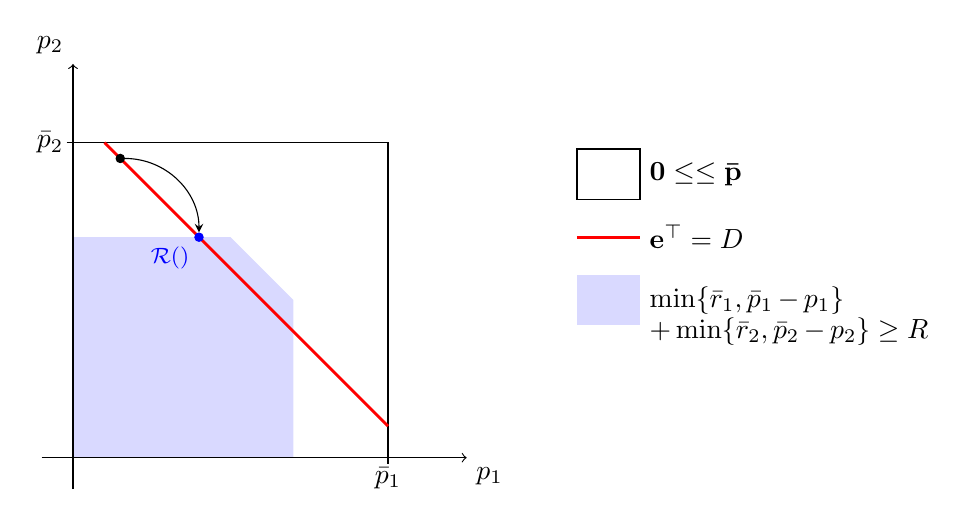
\begin{tikzpicture}[x=4cm,y=4cm]
        % X Axis
        \draw[black,->] (-0.1, 0.0) -- (1.25, 0.0);
        \node[below right] at (1.25, 0.0) {$p_{1}$};
            \draw[black] (1, -0.02) -- (1, 0.02);
            \node[below] at (1, 0.0) {$\bar{p}_{1}$};
        
        % Y axis
        \draw[black,->] (0.0, -0.1) -- (0.0, 1.25);
        \node[above left] at (0.0, 1.25) {$p_{2}$};
            \draw[black] (-0.02, 1) -- (+0.02, 1);
            \node[left] at (0, 1) {$\bar{p}_{2}$};
            
        % Reserve feasibility domain
        \fill[blue!50!white, fill opacity=0.3] (0,0) -- (0,0.7) -- (0.5, 0.7) -- (0.7, 0.5) -- (0.7, 0.0) -- cycle;
        
        % Domain of p1, p2
        \draw[black] (0,0) -- (0, 1) -- (1,1) -- (1,0) -- cycle;
        
        % Power balance constraint
        \draw[red,line width=1pt] (0.1, 1.0) -- (1.0, 0.1);
        
        % Infeasible prediction
        \node[circle,draw=black, fill=black, inner sep=0pt,minimum size=3pt] (phat_a) at (0.15, 0.95) {};
        \node[below left] at (0.15, 0.95) {\footnotesize $\pg$};
        
        % Feasible points of interest
        \node[circle,draw=blue, fill=blue, inner sep=0pt,minimum size=3pt] (pfeas1) at (0.4, 0.7) {};
        \node[below left, blue] at (0.4, 0.7) {\footnotesize $\mathcal{R}(\pg)$};
        
        \draw[-stealth] (phat_a.east) to [out=0,in=90] (pfeas1.north);
        
        % Legend
            % Domain of pg
            \draw[black] (1.6, 0.98) -- (1.8, 0.98) -- (1.8, 0.82) -- (1.6, 0.82) -- cycle;
            \node[right] at (1.8, 0.9) {$\mathbf{0} \leq \pg \leq \mathbf{\bar{p}}$};
            % Power Balance
            \draw[red, line width=1pt] (1.6, 0.7) -- (1.8, 0.7);
            \node[right] at (1.8, 0.7) {$\mathbf{e}^{\top} \pg = D$};
            % Reserve feasibility
            \fill[blue!50!white, fill opacity=0.3] (1.6, 0.58) -- (1.8, 0.58) -- (1.8, 0.42) -- (1.6, 0.42) -- cycle;
            \node[right] at (1.8, 0.5) {$\min\{\bar{r}_{1}, \bar{p}_{1} \, {-} \, p_{1}\}$};
            \node[right] at (1.8, 0.4) {$+\min\{\bar{r}_{2}, \bar{p}_{2} \, {-} \, p_{2}\} \geq R$};
    \end{tikzpicture}
    }
    \caption{Illustration of the reserve feasibility layer for $\mathbf{\bar{p}} {=} (1, 1)$, $\mathbf{\bar{r}}{=}(0.5, 0.5)$, $D {=} 1.1$, $R{=}0.8$ and the initial prediction $\pg {=} (0.15, 0.95)$. The recovered feasible dispatch is $\mathbf{\tilde{p}} {=} (0.4, 0.7)$.}
    \label{fig:feasibility_recovery:reserve}
\end{figure}
